\documentclass[12pt, utf8, hyperref]{article}
% \CTEXsetup[format={\Large\bfseries}]{section} %section标题左对齐
\usepackage{ctex}
\usepackage{graphicx}
\usepackage{float}
\usepackage{amsmath}
\usepackage{listings}
\usepackage{xcolor}

\hypersetup{
    colorlinks=true,
    linkcolor=black
} %set link in table of contents to black (default red)

\definecolor{vgreen}{RGB}{104,180,104}
\definecolor{vblue}{RGB}{49,49,255}
\definecolor{vorange}{RGB}{255,143,102}
\lstset
{
	basicstyle={\footnotesize\ttfamily},        % set code style
	keywordstyle=\color{vblue},
	identifierstyle=\color{black},
	commentstyle=\color{vgreen},
	% numbers=left,                      % set line numbers
	numberstyle={\tiny \color{black}}, % set fonts of line numbers
	frame=lines,                      % set type of open 
	numbersep=10pt,
	breaklines=true,                   % automatic line break
    tabsize=4,
    aboveskip=10pt,
    belowskip=2pt
}
% \setlength\parindent{0pt} %default no indent

\title{数值分析第一章实验报告}
\author{计65 \quad 王琛 \quad 2016011360}

\begin{document}
\maketitle

\section*{第1题}
\subsection*{1.解题思路}
计算出各个误差对应的数学表达式作为纵坐标,将h作为横坐标,在一张图中画出相应的曲线。根据泰勒展开,
\[
    f(x+h) = f(x)+hf'(x)+\frac{{h}^{2}}{2}f''(\xi) \quad \xi \in [x, x+h]
\]
\[
    f'(x) = 
    \frac{f(x+h)-f(x)-\frac{{h}^{2}}{2}f''(\xi)}{h}
\]
而近似方法$f'(x)=\frac{f(x+h)-f(x)}{h}$。因此近似算法的截断误差为$\frac{Mh}{2}$,其中M是$|f''(\xi)|$的上界,本题取1。舍入误差限为$\frac{2\epsilon}{h}$,其中$\epsilon$是数值误差的上界,本题中取$10^{-16}$。

因此总的误差限为两者之和,即
\begin{equation}
    \epsilon_{tot}=\frac{Mh}{2} + \frac{2\epsilon}{h}
\end{equation}

由于$f(x)=sinx$,$f'(x)=cosx$,matlab中$cosx$的计算可看成是精确的,因此当$x=1$时,实际总误差可写成:
\[ |cos1 - \frac{sin(1+h)-sin1}{h}|\]。

在matlab中画出每条线即可。

\subsection*{2.实验结果}
实验代码如下:
\begin{lstlisting}[language=matlab]
    h=logspace(-16,0,33);
    M=1;
    loglog(h,1/2.*M.*h);
    hold on
    loglog(h, eps/2./h);
    hold on
    loglog(h, 1/2.*M.*h + eps/2./h);
    hold on
    loglog(h, abs((sin(1+h)-sin(1))./h - cos(1)));
    hold on
    xlabel("步长h");
    ylabel("误差");
    title("不同步长取值对应的差商近似导数的误差");
\end{lstlisting}

所得的结果如下图所示:
\begin{figure}[H]
	\centering
	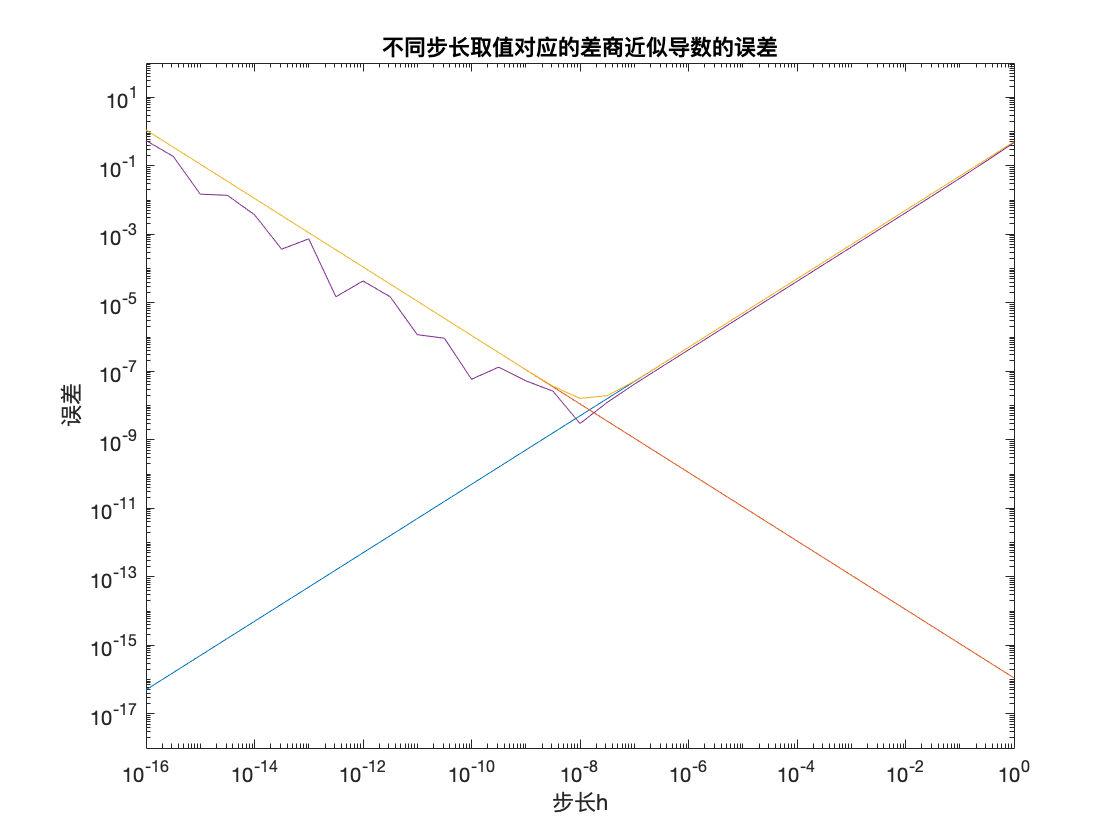
\includegraphics[scale=0.3]{../fig1.png}
	% \caption{Clusters got after k-means, points with the same color belong to one cluster}
	\label{Fig0}
\end{figure}

\subsection*{3.实验结论}
从图中可以看出,截断误差递增,舍入误差递减,总误差先减小后增大。根据等式(1),当$h=2\sqrt{\frac{\epsilon}{M}}=10^{-8}$时总计算误差最小,图中说明了这个结论。因此,我们在应用该方法计算时应该选取合适的h。

\section*{第3题}
\subsection*{1. 实验思路}
(1) 使用matlab的single命令转化为单精度浮点数,进入循环,每次加上$\frac{1}{n}$,当结果和上次循环相比不再变化时,退出循环。

(2) 使用(1)中求得的n进行循环,使用双精度。

\subsection*{2. 实验结果}
(1) 实验代码如下:
\begin{lstlisting}[language=matlab]
    n=0;
    tot = single(0);
    tot_prev = single(0);
    while true
        n = n + 1;
        tot = tot + single(1/n);
        if tot == tot_prev
            break;
        end
        tot_prev = tot;
    end
    disp("n=" + num2str(n) + " sum=" + num2str(tot));
\end{lstlisting}
输出为n=2097152 sum=15.4037。

(2) 代码如下:
\begin{lstlisting}[language=matlab]
    res = 0;
    tic
    for i=1:n-1
        res = res + 1/i;
    end
    toc
    disp("result with double float is " + num2str(res));
    disp("error="+num2str(tot-res));
\end{lstlisting}
输出为result with double float is 15.1333, error=0.27038。运行时间为0.003595s。

c++估算时间程序:
\begin{lstlisting}[language=c++]
    #include <iostream>
    #include <ctime>
    
    int main() {
        int n = 2097152;
        double res = 0;
        std::cout << CLOCKS_PER_SEC << std::endl;
        double begin = (double)clock();
        for(int i = 1; i <= n; i++) {
            res += 1/(double)n;
        }
        double end = (double)clock();
        std::cout << end - begin << std::endl;
        return 0;
    }
\end{lstlisting}

\subsection*{结果分析}
(1) 由定理1.6,当$|\frac{1/(n+1)}{\sum_{i=1}^{n}\frac{1}{n}}| <= \frac{1}{2}\epsilon_{mach}$时,出现抵消现象,结果不再变化。而单精度浮点数的机器精度为$2^{-24}=6.25*10^{-8}$,可写出如下程序进行粗略估计:
\begin{lstlisting}[language=matlab]
    sum=0;
    i=1;
    while(1/i/sum>0.5*6*10^(-8))
        sum=sum+1/i;
        i=i+1; 
    end
    disp(i);
\end{lstlisting}
估计出n=2113460时结果不再变化,与实验得到的n=2097152接近。

(2) n=2097152时,单精度结果为15.4037,双精度结果为15.1333,误差为0.27038,相对误差为1.79\%。

(3) 由于n趋向$\infty$时,$\sum\frac{1}{n} = lnn$,由定理1.6,$\frac{\frac{1}{n}}{lnn}<= 0.5*1.11*10^{-16}$,得出n约等于$5*10^{14}$。因n=2097152时,matlab时间为0.02587s且波动较大,c++时间为0.0062s, 采用c++的结果估算。当$n=5*10^{14}$时,时间为$\frac{0.0062*5*10^{14}}{2.1*10^{6}}=1.5*10^{6}s$,大概为17天。
\end{document}
